% =========================================================================== %

\begin{frame}[t,plain]
\titlepage
\end{frame}

% =========================================================================== %

\begin{frame}{Integration vs. Differentiation}
%
\begin{columns}
\column{.6\linewidth}
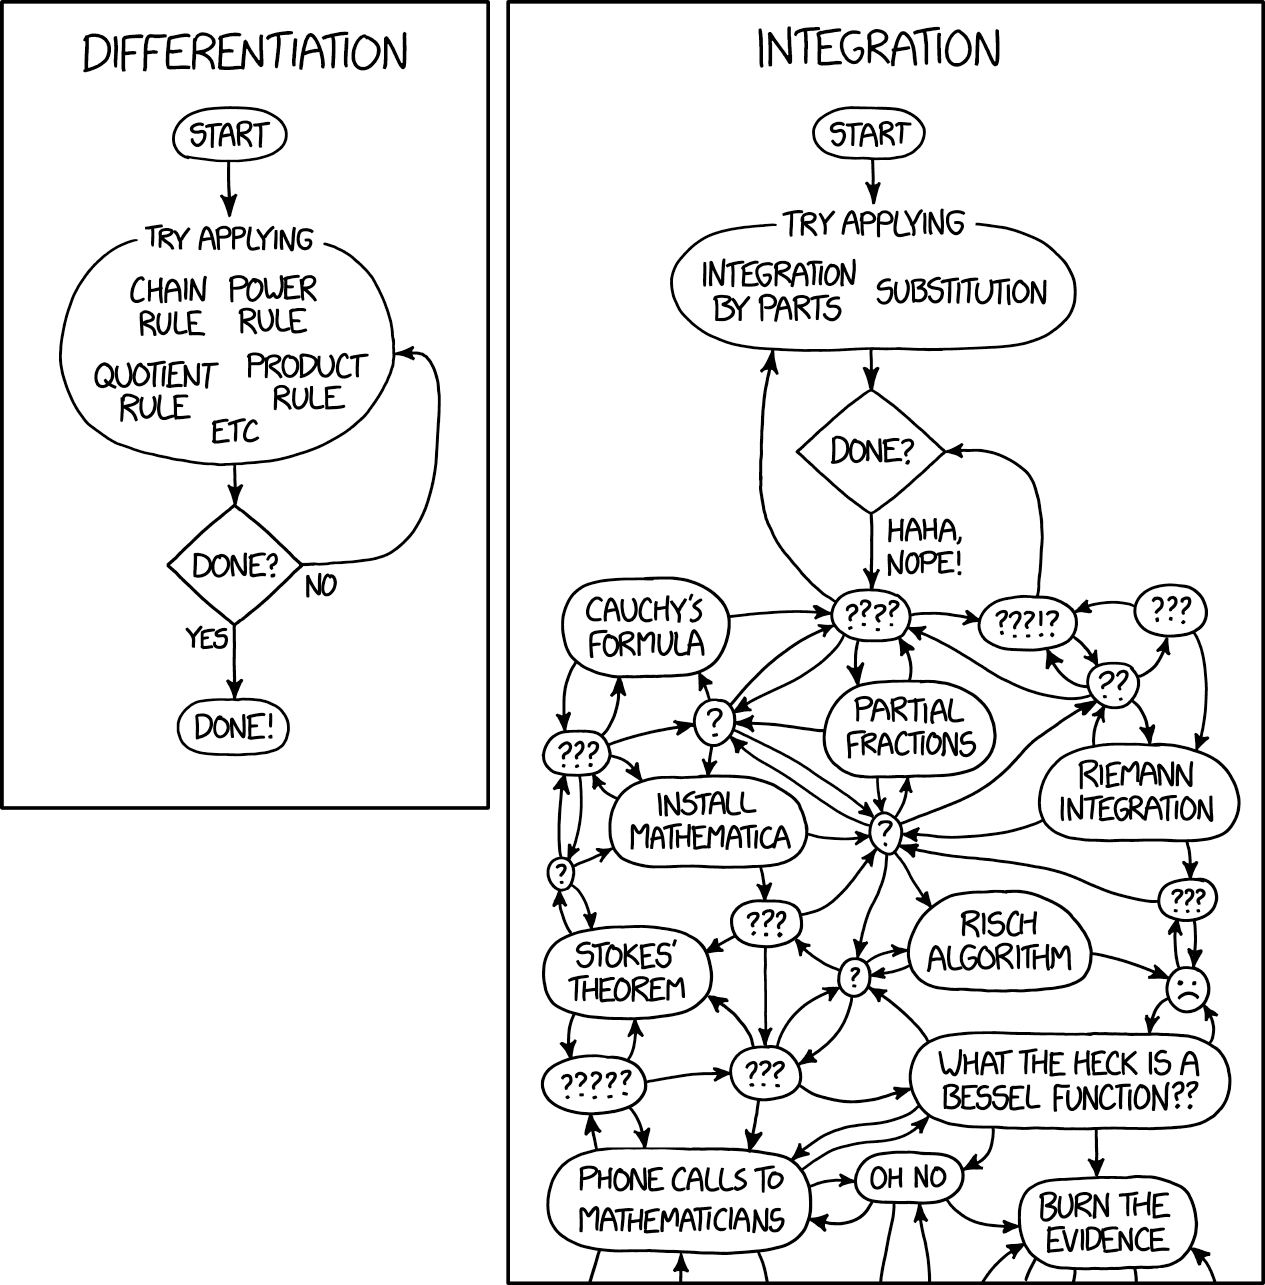
\includegraphics[width=.8\linewidth]{./gfx/03-xkcd-differentiation_and_integration}\\
%
\column{.3\linewidth}
\scriptsize
	\emph{\enquote{Symbolic integration} is when you theatrically go through the motions of finding integrals, 
		but the actual result you get doesn't matter because it's purely symbolic.}

	\vspace{6pt}
	\url{https://xkcd.com/2117/}
\end{columns}
%
\end{frame}

% =========================================================================== %

\begin{frame}{Scope for today}
%
\begin{itemize}
\item Numerical Derivatives
	\begin{itemize}
	\item Central difference method
	\item \texttt{numpy.gradient}
	\item (Higher order) derivatives by Convolution
	\end{itemize}
\item Integrals
	\begin{itemize}
	\item Given a callable
	\item Given an iterable
	\end{itemize}
\item Differential Equations
	\begin{itemize}
	\item First order
	\item Second and higher order
	\item Partial differential equations
	\end{itemize}
\end{itemize}
%
\end{frame}

% =========================================================================== %

\begin{frame}%{Derivatives}
%
\begin{defbox}[Definitions of Derivative]
\begin{align}
	\dv{x} f(x)
&=
	\lim_{\varepsilon \to 0}
		\dfrac{f(x + \varepsilon) - f(x)}{\varepsilon}
\\
	\dv{x} f(x)
&=
	\lim_{\varepsilon \to 0}
		\dfrac{f(x + \varepsilon) - f(x - \varepsilon)}{2\varepsilon}
\end{align}
\end{defbox}
%
\begin{itemize}
\item Standard Approach (1): Finite Differences: Set $\varepsilon$ to an arbitrary small but nonzero value
\item Works but error-prone
	\begin{itemize}
	\item Essentially amplified rounding errors
	\item Next Slides
	\end{itemize}
\item Small mitigation: central difference method (2)
	\begin{itemize}
	\item Improves the maths, not the rounding errors
	\end{itemize}
\end{itemize}
%
\end{frame}

% =========================================================================== %

\begin{frame}{Why The Central Difference Approximation Is More Accurate}
%
\begin{flalign}
\text{Taylor Expansion} \quad
&
	f(x + \varepsilon) 
~\approx~
	f(x) + f'(x) \varepsilon {\color{gray} + \dfrac{1}{2} f''(x) \varepsilon^2 + f'''(x) \varepsilon^3}
\\
\text{Implies} \quad
&
\dfrac
	{f(x + \varepsilon) - f(x)}
	{\varepsilon}
~\approx~
	f'(x) + 
	{\color{blue} \underbrace{\dfrac{1}{2} f''(x) \varepsilon}_{\mathcal{O}(\varepsilon)}} +
	{\color{gray} \dfrac{1}{6} f'''(x) \varepsilon^2}
	\label{eqn:forward-difference}
\\
\text{Likewise} \quad
&
	f(x - \varepsilon) 
~\approx~
	f(x) - f'(x) \varepsilon + {\color{gray} \dfrac{1}{2} f''(x) \varepsilon^2 - f'''(x) \varepsilon^3}
\\
\text{Implies} \quad
&
	\dfrac
		{f(x - \varepsilon) - f(x)}
		{\varepsilon}
~\approx~
	-f'(x) 
	{\color{blue}+\dfrac{1}{2} f''(x) \varepsilon}
	{\color{gray}
	 -\dfrac{1}{6} f'''(x) \varepsilon^2
	}\label{eqn:backward-difference}
\\
\text{Subtract (\ref{eqn:backward-difference}) from (\ref{eqn:forward-difference}) to get} \quad
&
\dfrac
	{f(x + \varepsilon) - f(x - \varepsilon)}
	{2\varepsilon}
~\approx~
	f'(x) 
	{\color{blue} + 0\varepsilon}
	+ \underbrace{
		\dfrac{1}{12} f'''(x) \varepsilon^2
	}_{\mathcal{O}(\varepsilon^2)} 
\end{flalign}
%
\end{frame}

% =========================================================================== %

\begin{frame}{Why This Won't Save Our Asses}
%
\begin{itemize}
\item IEEE 754: Standard for Floating-Point Arithmetic
	\begin{itemize}
	\item Institute of Electrical and Electronics Engineers (IEEE)
	\item Remember: only two symbols: 1 and 0. In particular, no comma
	\item Split bits in three parts: sign, mantissa, exponent
	\item Essentially: scientific notation: $0.0527 = 5.27 \cdot 10^{-2}$
	\item Mantissa: limited number of bits $\rightsquigarrow$ limited number of digits
	\item Rounding error when subtracting similar values
	\item Amplified when dividing by a small number
	\end{itemize}
\item No real way around this.
	\begin{itemize}
	\item Always be bad approximations for highly oscillatory functions
	\item Doesn't mean always bad
	\item But keep in mind to take derivatives with a grain of salt
	\end{itemize}
\item In particular bad for \emph{too small} values of $\varepsilon$.
	\begin{itemize}
	\item Python's \inPy{float} type allows ca. 15 significant digits
	\item $\varepsilon \approx 10^{-6}$ usually a good choice
	\end{itemize}
\end{itemize}
%
\end{frame}

% =========================================================================== %

\begin{frame}[fragile]{In Practice}
%
\begin{itemize}
\item Comparing derivative methods for $f(x) = \cos(\dfrac{1}{x^2 + c})$ with $c = 0.02$
	\begin{itemize}
	\item Ever faster oscillations closer to 0
	\item Control oscillation via $c$; smaller means faster
	\item Code for subsequent figures on GRIPS
	\item See \todo{specify location}
	\end{itemize}
\end{itemize}
%
\end{frame}

% =========================================================================== %

\begin{frame}{Comparing Methods}
%
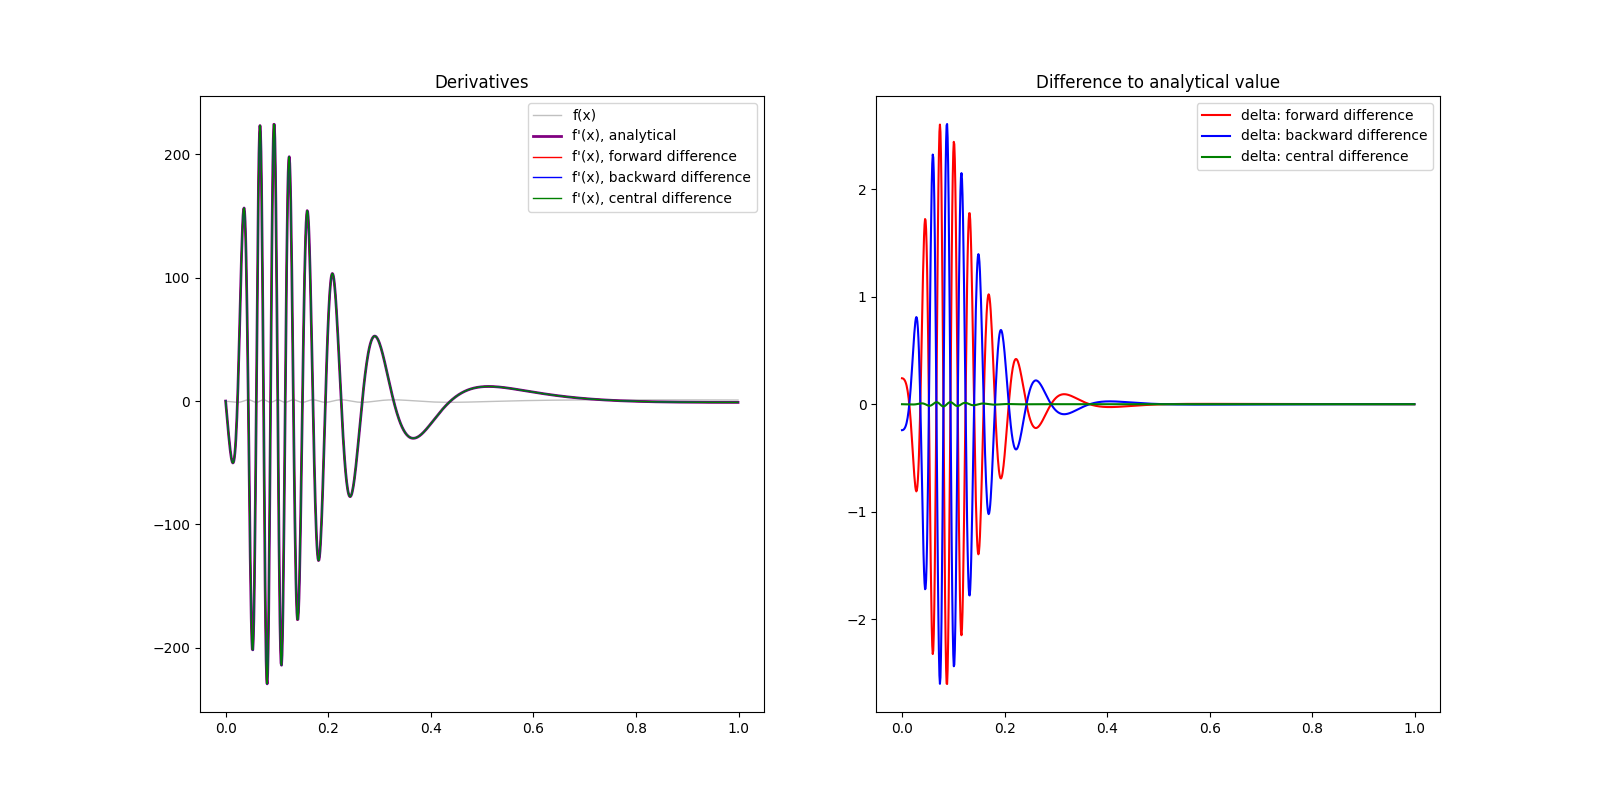
\includegraphics[width=\linewidth]{./gfx/03-derivative-methods}
%
\end{frame}

% =========================================================================== %

\begin{frame}{Comparing Epsilons}
%
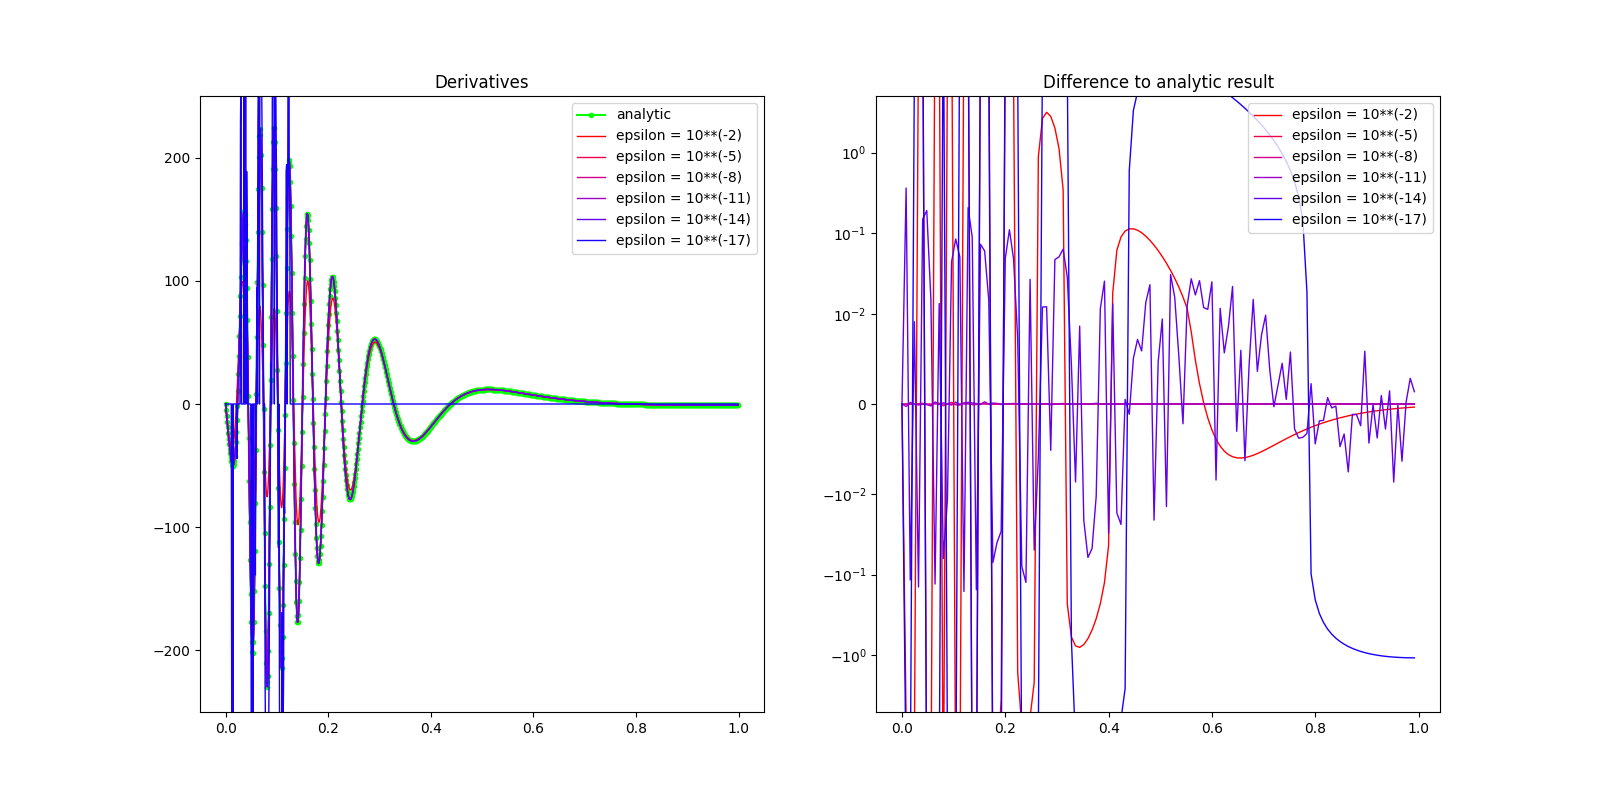
\includegraphics[width=\linewidth]{./gfx/03-derivative-epsilons}
%
\end{frame}

% =========================================================================== %


% picture from https://dsp.stackexchange.com/questions/27451/the-difference-between-convolution-and-cross-correlation-from-a-signal-analysis